%
% File emnlp2019.tex
%
%% Based on the style files for ACL 2019, which were
%% Based on the style files for EMNLP 2018, which were
%% Based on the style files for ACL 2018, which were
%% Based on the style files for ACL-2015, with some improvements
%%  taken from the NAACL-2016 style
%% Based on the style files for ACL-2014, which were, in turn,
%% based on ACL-2013, ACL-2012, ACL-2011, ACL-2010, ACL-IJCNLP-2009,
%% EACL-2009, IJCNLP-2008...
%% Based on the style files for EACL 2006 by 
%%e.agirre@ehu.es or Sergi.Balari@uab.es
%% and that of ACL 08 by Joakim Nivre and Noah Smith


\documentclass[11pt,a4paper]{article}
\usepackage[normalem]{ulem}
\usepackage{graphicx}
\useunder{\uline}{\ul}{}
\usepackage[hyperref]{emnlp-ijcnlp-2019}
\usepackage{times}
\usepackage{latexsym}
\usepackage{float}
\usepackage{multirow}

\usepackage{url}

\aclfinalcopy % Uncomment this line for the final submission

%\setlength\titlebox{5cm}
% You can expand the titlebox if you need extra space
% to show all the authors. Please do not make the titlebox
% smaller than 5cm (the original size); we will check this
% in the camera-ready version and ask you to change it back.

\newcommand\BibTeX{B{\sc ib}\TeX}

\title{Utilising Contextual Information to Improve Singular Word Correction}

\author{Nicholas Quek \\
  Computer Science Dept.\\
  University of Cambridge\\
  {\tt nq212@cam.ac.uk} }

\date{}

\begin{document}
\maketitle
\begin{abstract}
In computing, word correction is the process of providing suggestions for incorrectly spelled/used words in a text. Approaches to word correction have traditionally revolved around dictionaries. With the advent of machine learning, character and sub-word embedding have been developed to tackle this problem. These approaches, however, performs exceptionally poorly if the mistake is not close to the correct word. This paper employs a context-sensitive approach to tackle single word correction in order to overcome this limitation. Experiments conducted on a dataset gathered using multiple real English misspellings corpora showed an outstanding spelling error correction rate for mistakes which are far from its target.
\end{abstract}

\section{Introduction}

Errors in spelling may not pose a significant cognitive burden for a human reader. However, the restrictions they impose are amplified for an automated system. Automatic spelling correction is a required pre-processing component for many natural language processing (NLP) applications. Spelling correction is composed of two primary tasks, error detection and correction. This paper focuses solely on error correction, assuming that the offending word is identified in the input. 

This paper proposes the usage of Bidirectional Encoder Representations from Transformers (BERT) \cite{bert} to capture the word associations between the surrounding words and the offending word, in order to offer suggestions with a better semantic fit with the surrounding words. BERT is designed to produce deep bidirectional representations of text by jointly conditioning on both left and right context in all layers. \citet{bert} established that BERT produces state-of-the-art results on multiple NLP tasks, including sentence-level tasks, making it a perfect fit for context-sensitive spelling correction.

The proposed model achieved great accuracy for mistakes which are very different from the intended words. Its performance for smaller mistakes, however, is significantly worse compared to other spell checkers. This paper attempts an ensemble approach, integrating the model with ASpell. The ensemble approach captures the best of both text correctors, managing an acceptable correction rate for smaller mistakes while achieving exceptional accuracy, significantly beyond the other spell checkers (ASpell and Grammarly) used for comparison, for larger mistakes.

\section{Related Work}
Spelling error detection and correction is one of the key components in NLP systems, and many techniques have been developed since the 1960s. \citet{typesOfErrorDet} categorise spelling error correction algorithms under two broad umbrellas, isolated-word and context-dependent. 

Edit distance, proposed by \citet{editdistance}, is a popular isolated-word metric which is calculated on the number of operations to transform from the mistake to the suggested words. This metric is used to produce suggestions which the mistake could be a possible typo of. Learners of a language tend to spell unfamiliar words based on their pronunciations. Unfortunately, the spelling may be very different from the target, rendering edit distance ineffective. \citet{metaphone} proposed the metaphone algorithm which captures the pronunciation of words. The phonetic algorithm encodes words by reduction to sixteen consonant sounds. This bolster spell checkers' capabilities of matching words based on their phonetic similarity. More recently, neural word embedding for misspelled words was attempted. \citet{subwordembedding} discovered that the embedding efficiently reduced the search space for word suggestions. The reduction in search space meant that large edit distances mistakes were more likely to have valid corrections. 

The idea behind context-dependent approaches is to utilise words around the misspellings to provide semantic information. Language model-based approaches \cite{googleweb} utilising n-gram probabilities to incorporate context information is one such algorithm. Neural word embedding has also been used to capture sentence-level context of the misspelling. \citet{sentenceembedding} proposed combining the word embedding of individual words to create a context embedding. The vector operations used were basic (addition, multiplication, max embedding \cite{maxembedding}). The above machine-learning approaches have also been used in plenty of other NLP tasks. For example, both n-grams \cite{sentingram} and neural word embedding \cite{nnsenti} have been used for sentiment analysis. \citet{bert} proposed BERT which obtained new state-of-the-art results on eleven natural language processing tasks, including sentiment analysis. This paper attempts to leverage BERT to bolster contextual spell checkers' capabilities. 

\section{Approach}\label{approach}
This approach of this paper is to utilise a pre-trained BERT \cite{bert} model to capture the contextual information around the mistake (Section \ref{bert}). In Section \ref{fastText}, the misspelled word is vectorized into a sub-word embedding using a pre-trained fastText model \cite{fastText}. Next, we perform Principal Component Analysis (PCA) on the contextual embedding to reduce the input space (Section \ref{dimred}).  Both the reduced contextual embedding and the sub-word embedding are passed through a fully connected feed-forward neural network (Section \ref{ffnn}). The neural network outputs a sub-word embedding which we will compare with the embedding of words from the fastText vocabulary using nearest neighbours analysis to obtain suggestions (Section \ref{output}). Figure \ref{img:approach} provides the workflow for the approach this paper takes for spelling correction.

\begin{figure*}
\caption{Approach for spelling correction}
\centering
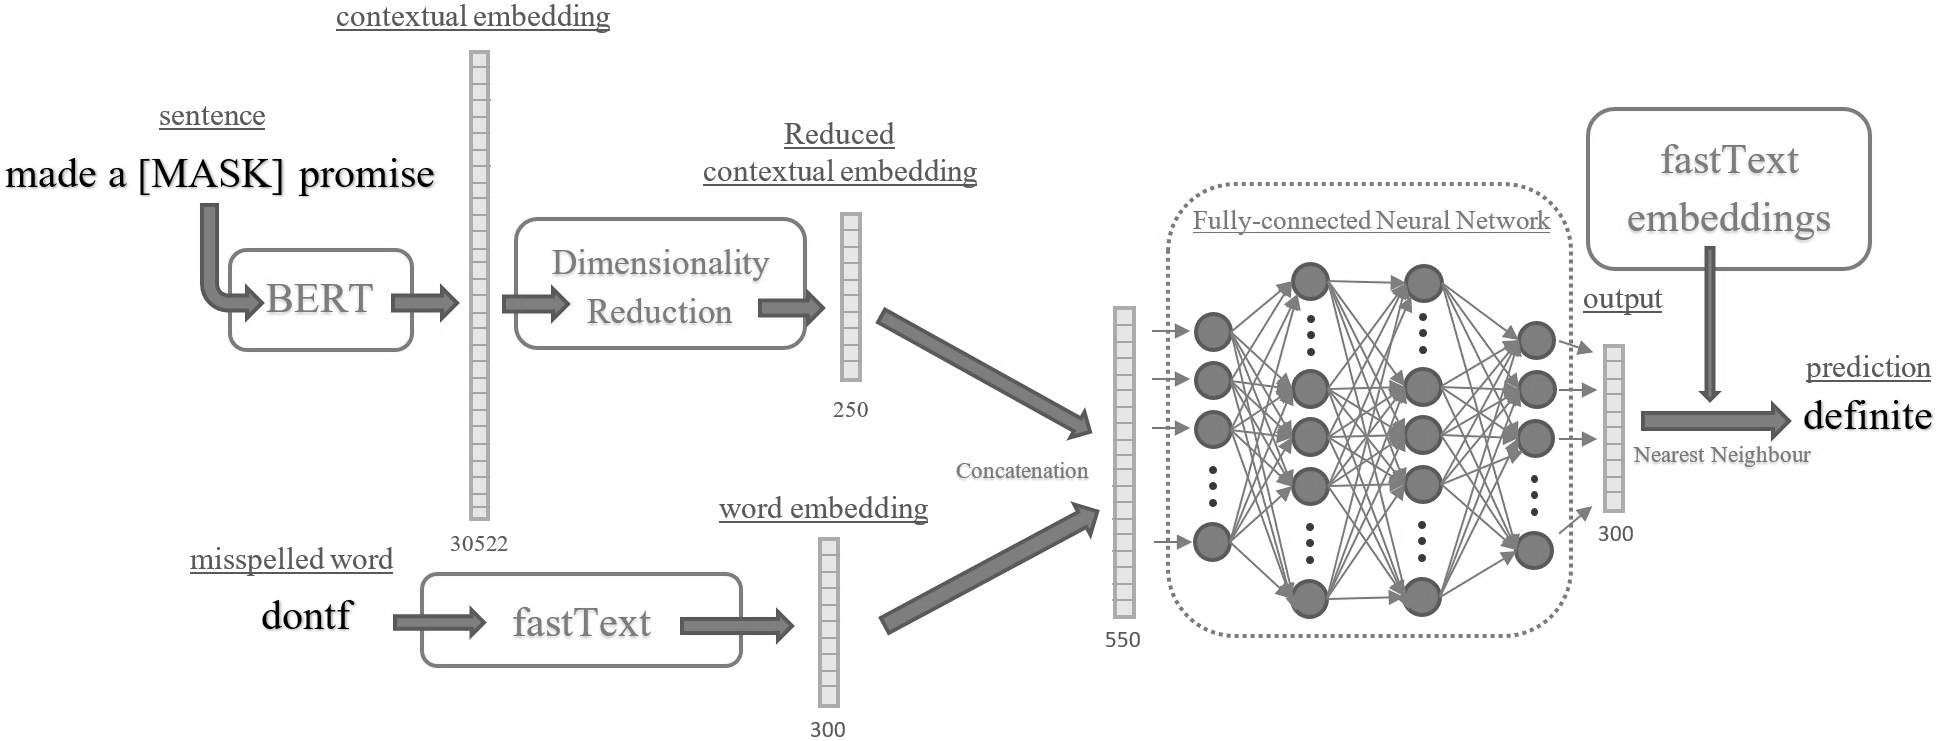
\includegraphics[width=16.4cm]{Flowchart_BW.jpg}
\label{img:approach}
\end{figure*}

\subsection{BERT}
\label{bert}
\citet{bert} introduced a general language modelling concept which facilities transfer learning and fine-tuning for specific NLP tasks. It quickly became the highlight by the end of 2018 for achieving state-of-the-art performance in many NLP tasks. 

For this paper, we focus on the feature extraction capabilities of BERT to obtain pre-trained representations of contextual information. BERT is trained with a masked language model objective. As a result, it is trivial to use BERT to capture contextual information around a selected word. We simply mask the word and input the sentence into BERT, which produces the contextual embedding.

BERT developers created two main models: BASE and LARGE. To reduce computational time, the BASE model was selected due to its significantly smaller footprint. The contextual embedding which is produced resides in a 30522-dimensional space. The large dimensionality proved difficult to work with. PCA (described in Section \ref{dimred}) was performed as an attempt to reduce the dimensionality. 

\subsection{fastText}
\label{fastText}
\citet{word2vec} introduced word2Vec, an approach which utilised either continuous bag-of-words (CBOW) or continuous skip-gram to obtain distributed representations of words. \citet{fastText} extended on this idea to create fastText. fastText attempts to introduce morphological information to the representations. Each word is represented as a bag of character n-grams (sub-words). The word2Vec algorithm is applied to the n-grams instead of words to obtain vector representations for each n-gram. A word is then represented as the sum of these individual n-gram vectors. fastText obtains better vectors for more uncommon complex words, even for out-of-vocabulary words, by looking at other words with similar morphology. This allow for the vectorization of misspellings which are often non-words.

For this paper, a pre-trained fastText model was used \cite{pretrainFTmodels}. This model was trained on Common Crawl and Wikipedia resources using CBOW with position-weights, with character n-grams of length 5, a window of size 5 and 10 negatives. The model outputs a 300-dimensional embedding. 

\subsection{Dimensionality Reduction}
\label{dimred}
Given a contextual embedding of dimension 30522, the number of tunable parameters for a fully connected feed-forward neural network with a single hidden layer is in excess of a hundred million. Tuning such a large parameter space would involve excessive data and time. 

To circumvent this, Principal Component Analysis was used to reduce the dimensionality. PCA is a statistical technique which utilises eigenvalue decomposition of a covariance (or correlation) matrix. It has the effect of concentrating much of the data into the first few features. While the later features may be dominated by noise, and can be removed without significant loss in data. 

Figure \ref{img:pca} shows the cumulative variance captured by the number of features. We observe that we require a much smaller set of features to capture a large portion of the variance. This is due to strong correlations between features within the initial set of 30522. We chose to reduce the dimensionality to 250, using the knee of the curve as a guide, striking a balance between capturing variance and reducing number of features.

\begin{figure}[H]
\caption{Principal Component Analysis}
\centering
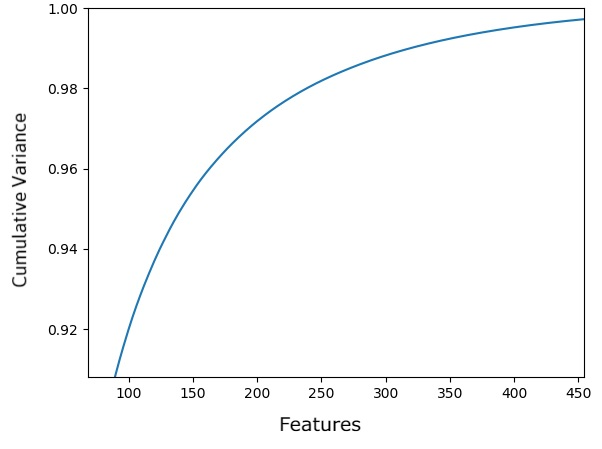
\includegraphics[width=7cm]{PCA.jpg}
\label{img:pca}
\end{figure}

\subsection{Fully connected Feed-forward neural network}
\label{ffnn}
We concatenate the reduced contextual embedding and the misspelled word embedding to produce a 550-dimensional vector which we use as input for the neural network. Selection of the parameters of the neural network is described in Section \ref{paramsel}. The output of the neural network is a 300-dimensional vector.

\subsection{Nearest Neighbours Analysis}
\label{output}
For qualitative analysis, the model needs to produce word suggestions for the misspelled word. Hence, the output of the neural network must be converted into suggestions. We search for the nearest neighbours according to cosine similarity among the vectors of the fastText model vocabulary. Cosine similarity is computed by calculating the dot product of the normalised vectors. This mechanism allows us to generate as many suggestions as required. However, the suggestions would come only from fastText vocabulary and the model would not be able to produce suggestions outside it.

\section{Dataset}
For simplicity, this paper focuses on single word errors. As such, word boundary errors such as agglutination (missing spaces between multiple words) and split errors (splitting a single word) caused by absent/misplaced white spaces are ignored. 

\citet{DataSpelling} gathered spelling errors corpora from multiple sources, including both native and non-native speakers corpora. This paper collates samples from the various misspelling corpora (APPLING, CHES, HOLBROOKS, NFER, PERIN, PETERS and WING) within Al-Jarf's corpora to create the dataset for training and evaluation purposes. Data from the CSpell training sets \cite{CSpell} were also taken to supplement the dataset. These corpora contained identified mistakes and their corrections as well as words surrounding the mistake. The examples from the corpora are further filtered to remove word boundary errors and possible duplicates. An additional step was also taken to remove all samples which contained ground truth words which are outside of the fastText vocabulary since the proposed mode would never provide the correct word. Samples containing characters which are not alphabetic characters, hyphens or apostrophes were also removed. In total, 7,382 data points were extracted from these sources. No fixed contextual window length was enforced, but the contexts are restricted to a sentence length (indicated by punctuation in the original samples). Some examples of the data points are as follows:
\begin{itemize}
  \item the boy threw a doatg \{dart\} 
  \item this is a missterticnic \{miscellaneous\} collection of goods
  \item there are also courses run to help you choose which kind of work suits you best and courses to train you for a particular job at operator or stem-skilled \{semi-skilled\} level
\end{itemize}

\citet{fourcontext} observed that most misspellings occur within a single edit distance. It is rare for misspellings to have large edit distances. Table \ref{Tab:EditDist} demonstrates the distribution of edit distances. For misspellings within small edit distances, contextual information is less relevant. In an attempt to amplify the effectiveness of contextual information, the dataset contain samples from very poor spellers and therefore contain a larger proportion of words which are very far away from their target.

\begin{table}[]
\caption{Edit Distance Distribution}
\begin{tabular}{l|llll}
Edit Distance & 1      & 2      & 3      & 4+     \\ \hline
{\ul }\citet{fourcontext} & 80.7\% & 13.7\% & 3.7\%  & 1.9\%  \\
This Paper & 27.8\% & 24.7\% & 20.0\% & 27.5\%
\end{tabular}
\label{Tab:EditDist}
\end{table}

\section{Experiments}\label{experiments}
A held-out test set was created using 10\% of the dataset. This test set is untouched until evaluation. The remaining data is split into five folds for cross-validation. 

Due to the output of the neural network being a 300-dimensional vector, there is a discrepancy between the loss function and evaluation metric. The evaluation metric for the model is the accuracy of the suggestions, which is the ratio of samples which the model makes the correct suggestions over total number of samples. The suggestions are produced using cosine similarity with word embedding from the fastText model. It is not immediately obvious how to compute gradients for this, resulting in it being ill-suited as a loss function. Instead, we use the fastText embedding, the 300-dimensional word embedding, of the correct word as the gold standard label for training. The loss is computed between the output and the gold label embedding and this loss is used as an approximation of the suggestion accuracy.

\subsection{Parameter Tuning}\label{paramsel}
The topology of the fully connected neural network consist of two hidden layers. The initial layer has 550 nodes to receive the 550-dimensional input. To allow for more complex interactions between the input features, the width of the first hidden layer is increased to 800. The second hidden layer is set to 500 to compress the features. The final layer outputs a 300-dimensional vector.

For training, the goal is to minimise the mean absolute error (MAE) objective. An adaptive moment estimation optimiser, Adam \cite{adam}, was used to update the network parameters. Mini-batch gradient descent was performed using a batch size of 10. Learning rate is set to 0.0001, with the exponential decay rate for the first and second moment fixed at 0.9 and 0.999 respectively. The training was regularised by weight decay (the L2 penalty multiplier set to 0.01) and dropout (ratio of 0.5) regularisation for all the hidden layers. The weight initialisation proposed by \citet{weights} was used with parameter set at $\sqrt{5}$.

A grid search was performed using five-fold cross-validation to select the above stated parameters. The model which was eventually selected was the one which achieved the highest suggestion accuracy on the validation set. The initial plan was to stop training once the validation loss stopped decreasing. In Figure \ref{img:losses}, the validation loss continued decreasing however the validation accuracy stopped increasing after epoch 1500. Since the loss function is only an approximation for the accuracy, the validation accuracy was used to determine when to stop training.

\begin{figure}[H]
\caption{Validation Loss and Accuracy}
\centering
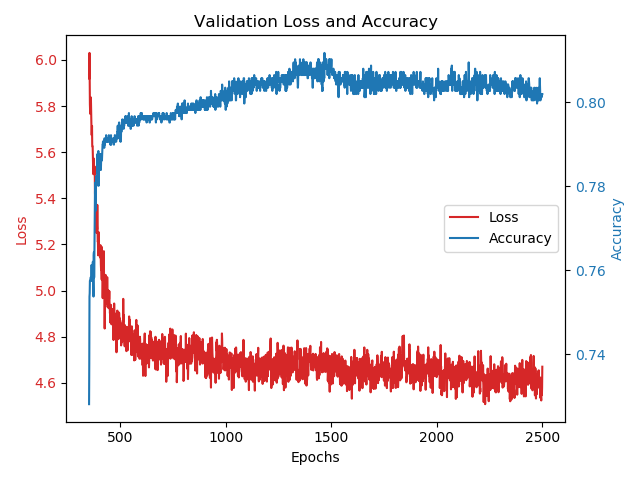
\includegraphics[width=7.5cm]{Epochs.png}
\label{img:losses}
\end{figure}

\section{Evaluation and Discussion}
\subsection{Performance of mistake embedding} \label{individualemb}
In Section \ref{fastText}, we used a pre-trained fastText model to obtain the embedding for the misspelled word. An investigation was conducted to observe the performance of the mistake embedding in isolation. The embedding were used to generate suggestions using nearest neighbours and the top ten predictions were considered during the evaluation of the held-out test set. 

Table \ref{Tab:purecompare} display the results for the mistake embedding as well as the performance of the proposed model which combines the mistake embedding with contextual information using a fully connected neural network. 

\begin{table}[H]		
\caption{Accuracy of the top ten corrections using embedding in isolation}
\begin{tabular}{l|llll}
           & \multicolumn{4}{l}{Edit Distance} \\ \cline{2-5} 
           & 1      & 2      & 3      & 4+     \\ \hline
Mistake Em & \textbf{62.8\%} & 16.9\% & 4.58\% & 0.57\%    \\
This Paper & 54.8\% & \textbf{85.9\%} & \textbf{91.7\%} & \textbf{87.4\%}  
\end{tabular}
\label{Tab:purecompare}   
\end{table}

The mistake embedding provides better suggestions for small edit distance mistakes but performs poorly for large distances due to the larger search space. In contrast, the model performs poorer compared to the mistake embedding for small edit distances but significantly better for large edit distances. This agrees with the intuition that contextual information would be a good heuristic to utilise for correction of large edit distance mistakes, where the misspelled word does not provide a good starting point for suggestions.

The proposed model which combines both mistake and contextual embedding managed to produce suggestions which were remarkably superior for large edit distance mistakes. However, simply using the mistake embedding achieves better suggestions for small edit distances. The poorer performance of the model on small edit distance mistakes hints at over-reliance on contextual information. 

\subsection{Trade-off between mistake and contextual information}\label{tradeoff}
In Section \ref{individualemb}, the question of whether contextual information is being overly exploited and this has degraded the text corrections for smaller edit distance mistakes was raised. An experiment was performed to verify if such a trade-off exists. 

ASpell has different suggestion modes. One of them is the bad spellers mode.
This mode utilises an n-gram scan which is tailored towards the bad speller. The other modes attempt to strike a good balance between typos and true misspellings. In contrast, the bad spellers mode does not perform typo-analysis and is more likely to return positive suggestions if the misspelled word looks anything like the correct spelling. Table \ref{Tab:ASpell} captures the performance of Aspell default and the bad spellers mode. It evaluates their accuracy based on the top k suggestions each mode provides for different values of k.

\begin{table*}[]
\caption{Accuracy of the top k corrections of two ASpell modes}
\centering
\begin{tabular}{c|l|llll}
\multicolumn{1}{l|}{\multirow{2}{*}{Top k Suggestions}} & \multirow{2}{*}{Suggestion Mode} & \multicolumn{4}{l}{Edit Distance} \\ \cline{3-6} 
\multicolumn{1}{l|}{}                                   &                                  & 1      & 2      & 3      & 4+     \\ \hline
\multirow{2}{*}{10}                                     & Default                          & 97.7\% & 66.2\% & 42.7\% & 21.2\% \\
                                                        & Bad Spellers                     & 93.0\% & 66.9\% & 42.0\% & 22.4\% \\ \hline
\multirow{2}{*}{20}                                     & Default                          & 98.5\% & 73.2\% & 48.9\% & 24.7\% \\
                                                        & Bad Spellers                     & 95.3\% & 74.6\% & 51.1\% & 31.0\% \\ \hline
\multirow{2}{*}{100}                                    & Default                          & 99.2\% & 76.1\% & 51.1\% & 26.4\% \\
                                                        & Bad Spellers                     & 99.2\% & 92.3\% & 70.2\% & 43.1\%
\end{tabular}
\label{Tab:ASpell}   
\end{table*}

From Table \ref{Tab:ASpell}, the performance of the two modes does not vary significantly from each other when only ten suggestions are considered. The search space for large edit distance mistakes is likely to be larger than ten and therefore has not been explored significantly. When the number of considered suggestions is large (100), the performance of the bad spellers significantly overwhelms the default mode. The search space for small edit distance mistakes is likely to be fully explored given a hundred suggestions. Therefore, there is no degradation in performance, while the contextual information captured by n-grams plays its role to boost performance for large edit distance mistakes. 

We observe a more representative trade-off when the number of suggestions is twenty. At twenty suggestions, there is a trade-off in the performance for small and large edit distance mistakes. The lack of typo-analysis in the bad spellers mode is likely causing the smaller edit distance mistakes to be corrected less frequently compared to the default mode. The search space, though small, is likely not to be been fully explored with only twenty suggestions. The utilisation of n-gram scan improves the performance on larger edit distance mistakes. The trade-off between accuracy for the different mistakes agrees with our hypothesis that the proposed model is indeed relying too heavily on contextual information to form its suggestions. 

\subsection{Comparison with other Spell Checkers} \label{otherspellcheckers}
For a more thorough evaluation of the proposed model, we would be comparing its performance against other spell checkers. GNU Aspell \cite{Aspell} and Grammarly \cite{Grammarly} were used.

GNU Aspell is an open source cross-platform spell checker that has become the standard spell checker for the GNU software project. Commercial software applications such as Notepad++ and gedit have also integrated it into their functionalities. The feature that allows it to stand out among other spell checkers is its superior replacement suggestions for misspelled words. Although first released in 2010, it has been regularly maintained and refined. The latest update (at the moment of writing) was in Oct 2019. 

Grammarly is a proprietary contextual spell checker developed by Grammarly Inc. It is built to analyse English sentences, taking context into account when making corrections or suggestions. The outstanding spelling correction tool has garnered popularity over the years, boasting more than 20 million daily active users in Oct 2019. 

Since we are evaluating only spelling correction capabilities, the test set is trimmed to only include samples whose mistakes can be detected by both spell checkers, resulting in a test set of 576 data points. Table \ref{Tab:SpellCheckResults} contains the accuracy of the various spell checkers, taking into account their top three predictions for the misspelled word. For the case of Grammarly, there are situations where the spell checker correctly identified the misspelling but is unable to provide a suggestion. The evaluation recognised these cases as a failure to provide the correct suggestion. 

\begin{table}[]		
\caption{Accuracy of the top three corrections of various spell checkers}
\begin{tabular}{l|llll}
           & \multicolumn{4}{l}{Edit Dist} \\ \cline{2-5} 
           & 1      & 2      & 3      & 4+     \\ \hline
ASpell     & 84.5\% & 54.2\% & 31.3\% & 13.2\%    \\
Grammarly  & \textbf{97.7\%} & 84.5\% & 64.9\% & 0.00\%  \\
This Paper & 55.8\% & \textbf{85.9\%} & \textbf{90.8\%} & \textbf{88.5\%}     
\end{tabular}
\label{Tab:SpellCheckResults}   
\end{table}

Surprisingly, the contextual spell checker, Grammarly, performed terribly on large edit distance mistakes. Grammarly was unable to correctly suggest word corrections for even one of the 174 mistakes with distances larger than 3. However, Grammarly's performance for the smaller distances were clearly superior amongst the spell checkers. 

The proposed model performance for the large distances are great, achieving an accuracy of 88.5\% for mistakes with distances beyond three, compared to 13.2\% using ASpell and 0.0\% using Grammarly. However, the performance for mistakes of distance one away from their target is significantly poorer compared to the others. It achieved an accuracy of 55.8\% compared to the 84.5\% of ASpell and 97.7\% of Grammarly. This poor accuracy is unacceptable, considering the distribution of mistakes in practice as shown in Table \ref{Tab:EditDist}. To address the poor accuracy, we attempt to utilise the typo-analysis algorithms utilised by ASpell using an ensemble approach (Section \ref{ensemble}).

\subsection{Ensemble approach}\label{ensemble}
In Section \ref{tradeoff}, we experimented using a larger number of suggestions to see their impact on text correction. However, in practice, suggesting more than three corrections would overwhelm the user. Given a constraint of three suggestions, we want to achieve an appropriate trade-off between typo-analysis and utilising contextual information. \citet{reranking} proposed a strategy of using a re-ranking model to re-rank suggestions. While more complicated strategies can be used, this paper employs a trivial combination of suggestions, taking the top two suggestions from ASpell and the best from the proposed model. Table \ref{Tab:rerank} shows the performance of this simple ensemble approach. This approach capitalises on the strengths of both spell checkers, to significantly boost performance for both small and large edit distance mistakes. The ensemble approach is able to utilise the developed typo-analysis algorithms for the more common smaller edit distance mistakes, while able to utilise contextual information to provide suggestions for when the mistake is far from the target word.  

\begin{table}[H]		
\caption{Accuracy of the top three corrections}
\begin{tabular}{l|llll}
           & \multicolumn{4}{l}{Edit Distance} \\ \cline{2-5} 
           & 1      & 2      & 3      & 4+     \\ \hline
ASpell     & 84.5\% & 54.2\% & 31.3\% & 13.2\% \\
Grammarly  & \textbf{97.7\%} & 84.5\% & 64.9\% & 0.00\%  \\
This Paper & 55.8\% & 85.9\% & 90.8\% & 88.5\% \\
Ensemble   & 86.0\% & \textbf{92.3\%} & \textbf{96.2\%} & \textbf{92.0\%}
\end{tabular}
\label{Tab:rerank}   
\end{table}

The ensemble approach achieves superior results, a 30.2\% boost in accuracy compared to the original model performance for small edit distance mistakes. It achieves the best of both worlds, using typo-analysis to generate suggestions which are close to the mistake and contextual information for suggestions further from the mistake. This combination of both techniques achieves 86.0\% accuracy for mistakes with edit distances of one, only lower than Grammarly performance. The ensemble achieves accuracy of 92.0\% for distances beyond three, a full 75\% of accuracy over the other spell checkers. 

\section{Future Work}
Due to time limitations, not all aspects of the project were thoroughly explored. In Section \ref{otherspellcheckers}, we identified that performance of the proposed model is lacking when handling small edit distance mistakes. There is an underlying concern that the training set being skewed in its edit distance distribution is likely causing the model to place excessive emphasis on contextual information. A more realistic distribution for the training set would likely generate a model which handles small edit distance mistakes better. However, the trade-off between the distances would likely remain. A deeper investigation would require a more realistic and comprehensive training set. 

Alternatively, the ensemble approach taken by this paper (Section \ref{ensemble}) could also address the poor performance. The paper uses a trivial combination of suggestions from ASpell and the heavily emphasised contextual model to achieve a balance between both small and large edit distance mistakes. More sophisticated re-ranking architectures could be designed to fully capitalise on the advantages of both Aspell and the proposed contextual spell checker. \citet{CSpell} utilises a multi-layer correction model design resembling a pipeline, where different corrector models generate suggestions and rankers rank the suggestions appropriately. The proposed context-sensitive text corrector could be used as a correction module in this pipeline to incorporate contextual information into the correction decision.   

A crucial aspect of text correction which this paper did not address is the speed. The process of using multiple neural networks for encoding and processing is slow. More work would need to be done to optimise this process. For example, using approximation techniques for the BERT and fastText models to simplify the encoding process.

\section{Conclusion}
We developed a context-sensitive text correction model for correction of spelling errors. The approach utilises BERT and fastText to generate state-of-the-art embedding for contextual information and out-of-vocabulary words. A fully connected neural network is employed to integrate these embedding to generate predictions for spelling errors. The combination of these embedding performed exceptionally well for large edit distance mistakes. However, there was an unexpected trade-off in its performance for smaller edit distance mistakes. The paper then proposes an ensemble approach which reduces the emphasis on contextual information to achieve a balance between the performances for mistakes of different distances. The software, training and testing data are available on GitHub.


\bibliography{emnlp-ijcnlp-2019}
\bibliographystyle{acl_natbib}

\end{document}
